\documentclass[conference]{IEEEtran}

\usepackage[utf8]{inputenc}
\usepackage{tikz}
\usepackage{graphicx}
\usepackage{float}
\usepackage{hyperref}
\usetikzlibrary{shapes.geometric, positioning, arrows.meta, backgrounds, fit}

\title{PharmAssist -- Smart Voice \& Text Agent for Pharmacy Assistance: \\
Exhaustive System Architecture and Component Analysis}

\author{
\IEEEauthorblockN{Mihir}
\IEEEauthorblockA{
M.Tech Major Project Report\\
Department of Computer Science\\
[University Name]\\
[City, Country]\\
email@domain.com}
}

\begin{document}

\maketitle

\begin{abstract}
This report provides an in-depth, highly technical breakdown of PharmAssist -- Smart Voice \& Text Agent for Pharmacy Assistance, an autonomous AI-powered conversational agent engineered specifically for the retail pharmacy sector. The system is designed to seamlessly handle concurrent customer interactions regarding medication availability, reservations, pricing, and pharmacological advice over standard telephone networks. By relying on a high-performance streaming architecture, PharmAssist utilizes FastAPI for asynchronous event routing, Twilio for telephony bridging, Deepgram for real-time streaming Speech-to-Text (STT), ElevenLabs for ultra-low latency Text-to-Speech (TTS) synthesis, and a sophisticated LangGraph-based agentic workflow driven by Google's Gemini 2.5 Pro LLM. This document exhaustively explains the internal mechanics, network protocols, tool execution flows, ACID-compliant database state management, and the integrated administrative dashboard, providing a complete blueprint of a modern voice AI pipeline.
\end{abstract}

\section{Introduction and Problem Statement}
In the modern healthcare ecosystem, retail pharmacies serve as a critical bridge between clinical prescriptions and patient wellness. However, these facilities face a significant operational bottleneck: the sheer volume of routine, repetitive inquiries made over the phone. Patients constantly call to verify if a specific drug is in stock, inquire about business hours, ask for pricing on generic alternatives, or seek advice regarding medication side effects. Consequently, highly trained pharmacists are frequently interrupted from critical clinical duties simply to answer trivial logistical questions. 

Historically, the telecommunications and software industries attempted to solve this issue through Interactive Voice Response (IVR) systems. Traditional IVRs operate on rigid, deterministic, state-machine-driven decision trees (e.g., "Press 1 to check stock"). These systems suffer from a fatal flaw: they completely lack Natural Language Understanding (NLU), leading to extreme user frustration and high call abandonment rates.

The PharmAssist system represents a paradigm shift from rigid decision trees to Generative AI "Agentic Workflows." Unlike early-generation chatbots that rely on simple keyword matching, PharmAssist utilizes advanced Large Language Models capable of maintaining deep contextual awareness. It can understand highly nuanced, multi-part, spoken queries, autonomously decide to fetch real-time data from an inventory database, execute state-altering transactions, and synthesize a response in a natural, empathetic human voice. 

\section{High-Level Architecture and The Latency Budget}
Designing a voice bot requires solving a fundamental physics problem: the latency budget. In natural human conversation, the acceptable gap between one person finishing a sentence and the other person beginning their reply is generally between 500 to 1200 milliseconds. Because traditional HTTP REST APIs require opening and closing connections for every single request, they introduce too much network overhead to meet this strict latency budget. Therefore, the entire PharmAssist architecture is event-driven and built upon \textbf{WebSockets}---a protocol that provides full-duplex, continuous communication channels over a single TCP connection. 

\begin{figure}[H]
\centering
\resizebox{\columnwidth}{!}{
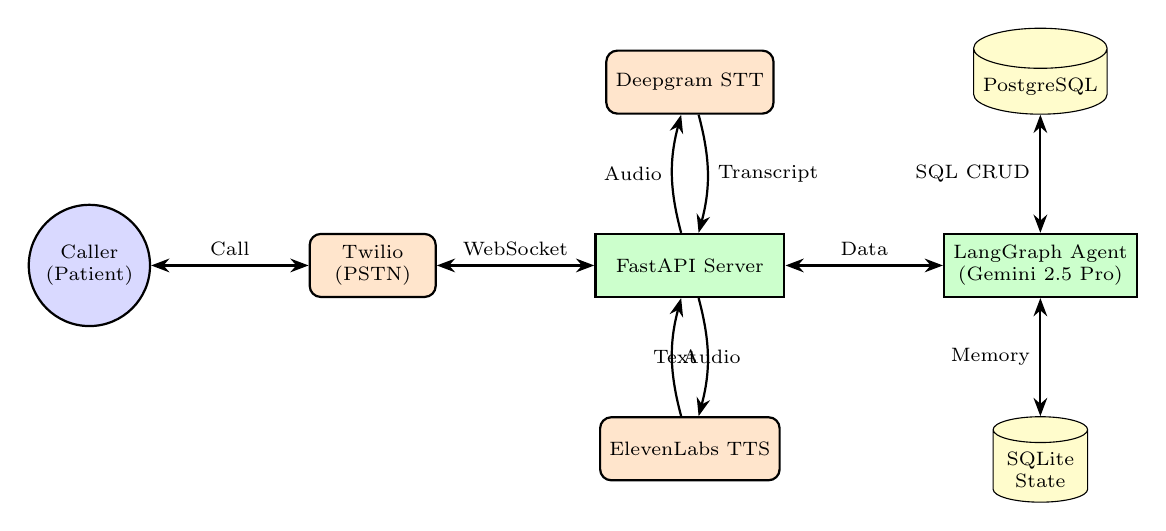
\begin{tikzpicture}[
node distance=1.5cm and 2cm,
>=Stealth,
every node/.style={font=\scriptsize},
user/.style={circle, draw, thick, fill=blue!15, minimum size=1cm, align=center},
service/.style={rectangle, rounded corners, draw, thick, fill=orange!20, minimum width=1.6cm, minimum height=0.8cm, align=center},
core/.style={rectangle, draw, thick, fill=green!20, minimum width=2.4cm, minimum height=0.8cm, align=center},
database/.style={cylinder, draw, shape border rotate=90, aspect=0.3, minimum height=0.8cm, minimum width=1.2cm, fill=yellow!20, align=center},
line/.style={->,thick},
bline/.style={<->,thick}
]

% Nodes
\node[user] (caller) {Caller\\(Patient)};
\node[service, right=of caller] (twilio) {Twilio\\(PSTN)};
\node[core, right=of twilio] (fastapi) {FastAPI Server};
\node[service, above=of fastapi] (deepgram) {Deepgram STT};
\node[service, below=of fastapi] (eleven) {ElevenLabs TTS};
\node[core, right=of fastapi] (agent) {LangGraph Agent\\(Gemini 2.5 Pro)};
\node[database, above=of agent] (db) {PostgreSQL};
\node[database, below=of agent] (sqlite) {SQLite\\State};

% Connections
\draw[bline] (caller) -- node[above]{Call} (twilio);
\draw[bline] (twilio) -- node[above]{WebSocket} (fastapi);
\draw[line] (fastapi) to[bend left=15] node[left]{Audio} (deepgram);
\draw[line] (deepgram) to[bend left=15] node[right]{Transcript} (fastapi);
\draw[line] (fastapi) to[bend left=15] node[left]{Text} (eleven);
\draw[line] (eleven) to[bend left=15] node[right]{Audio} (fastapi);
\draw[bline] (fastapi) -- node[above]{Data} (agent);
\draw[bline] (agent) -- node[left]{SQL CRUD} (db);
\draw[bline] (agent) -- node[left]{Memory} (sqlite);

\end{tikzpicture}
}
\caption{System Architecture Flow}
\label{fig:architecture}
\end{figure}

\section{Exhaustive Component Breakdown}

\subsection{Telephony and Asynchronous WebSocket Server}
The physical bridge between the telecommunications network and the software stack is Twilio. When a user dials the pharmacy's provisioned Twilio phone number, Twilio intercepts the PSTN signal and makes an HTTP POST request to a webhook hosted on our backend server. The server responds with TwiML (Twilio Markup Language), specifically instructing Twilio to initiate a \texttt{<Stream>} command. This command opens a bidirectional WebSocket connection directly to the server.

Once the socket is open, Twilio begins pushing audio payloads. To ensure compatibility with telecom standards and minimize bandwidth, the audio is encoded in \textbf{G.711 $\mu$-law} format at an \textbf{8000Hz sampling rate}. 

To handle this continuous influx of audio bytes from potentially dozens of concurrent callers, the backend is built on \textbf{FastAPI} running atop an ASGI server (Uvicorn). FastAPI utilizes Python's \texttt{asyncio} event loop. This allows the server to act as a highly efficient traffic controller---instantly piping incoming audio bytes to the Speech-to-Text engine, and feeding returning audio bytes from the Text-to-Speech engine back into the Twilio socket, all without dropping a single frame of data.

\subsection{Speech-to-Text (STT) Engine: Deepgram and VAD Endpointing}
To transcribe human speech into text instantaneously, the FastAPI server opens a secondary persistent WebSocket connection to Deepgram's streaming API. Deepgram utilizes specialized neural network architectures optimized specifically for streaming transcription.

The most complex engineering challenge in streaming voice AI is determining exactly \textit{when} the user has finished speaking so the AI can formulate a response (turn-taking). To solve this, PharmAssist relies on Deepgram's \textbf{Voice Activity Detection (VAD) endpointing}. The system is strictly configured to monitor the audio stream for a continuous \textbf{500-millisecond window of absolute silence}. When this threshold is met, Deepgram emits a \texttt{speech\_final} flag alongside the text transcript. The FastAPI server captures this flag and instantly passes the finalized text to the AI Agent.

\subsection{Cognitive Reasoning Engine: Gemini 2.5 Pro and LangGraph}
The absolute core of the PharmAssist cognitive pipeline is the \textbf{LangGraph ReAct (Reasoning and Acting) Agent}, powered specifically by \textbf{Google's Gemini 2.5 Pro} Large Language Model.

\textbf{Why Gemini 2.5 Pro?}
Gemini 2.5 Pro was selected as the foundational LLM for this project due to its exceptional capabilities in tool-calling, vast context window, and ultra-fast inference speeds. Voice agents require an LLM that can not only parse natural language but deterministically output structured JSON commands to execute Python functions. Gemini 2.5 Pro excels in these agentic workflows, ensuring that reasoning loops execute almost instantaneously without compromising on logical accuracy.

\textbf{The LangGraph Reasoning Loop}
Traditional LLM pipelines are linear (User Input $\rightarrow$ Prompt $\rightarrow$ Output). LangGraph, however, structures the Gemini LLM's logic as a cyclic graph. When the finalized transcript is received, the agent enters a rigorous loop:
\begin{enumerate}
    \item \textbf{Observe:} Gemini analyzes the user's current spoken intent alongside the entire past conversation history (e.g., resolving pronouns like "I'll take \textit{it}").
    \item \textbf{Reason:} Gemini evaluates if it has enough internal knowledge to reply directly, or if it must query the external database to verify facts (e.g., checking if a specific medicine is currently in stock).
    \item \textbf{Act:} If external data is required, Gemini generates a structured JSON payload that triggers a deterministic Python function (a Tool). The agent then waits for the tool to execute, ingests the resulting data, and loops back to the "Reason" phase to decide if more tools are needed or if it is ready to formulate a spoken response.
\end{enumerate}

This cyclical logic allows the Gemini agent to safely navigate highly ambiguous human queries. For example, if a user asks to reserve "Paracetamol," the agent queries the database and realizes there are multiple manufacturers available. Instead of guessing, Gemini halts the reservation tool, verbally lists the available options to the user, and waits for verbal clarification before finalizing the order.

\subsection{Text-to-Speech (TTS) Engine: ElevenLabs}
Once the Gemini agent finalizes its textual response, the text is routed via HTTP to ElevenLabs. ElevenLabs utilizes proprietary voice cloning and synthesis neural networks capable of conveying complex human emotion, natural intonation, and realistic pacing. To completely eliminate transcoding latency on our server, the API is explicitly instructed to return audio natively in the \texttt{ulaw\_8000} format, which is immediately pushed into the Twilio WebSocket.

\section{Tool Calling Integrations and Database Integrity}
Large Language Models are probabilistic engines; they are mathematically prone to "hallucinations." In a healthcare setting, hallucinating inventory or medical advice poses severe ethical risks. Therefore, the Gemini 2.5 Pro LLM is highly restricted. It cannot invent facts; it must rely strictly on deterministic Python tools to fetch hard data.

\subsection{Inventory and Order Tools}
\begin{itemize}
    \item \textbf{Search Medicine Tool:} When a user asks about a drug, the Gemini agent executes a secure SQL \texttt{ILIKE} pattern-matching query against the PostgreSQL database, returning exact stock counts, manufacturers, and active prices directly to the LLM's context window.
    \item \textbf{Reserve Medicine Tool:} This tool accepts the caller's phone number, the requested medicine ID, and the quantity. Crucially, it features \textbf{atomic stock deduction} logic implemented via SQLAlchemy. PharmAssist utilizes database row-locking; the transaction locks the inventory row, verifies the stock is still greater than zero, deducts the quantity, and writes a persistent Reservation record tied to the user's caller ID. If the stock is insufficient, the transaction rolls back, and Gemini informs the caller.
\end{itemize}

\subsection{Retrieval-Augmented Generation (RAG)}
When a patient asks a pharmacological question (e.g., "Can I take Ibuprofen on an empty stomach?"), the agent executes a specialized RAG tool to prevent medical hallucination. The RAG tool converts the user's natural language question into a high-dimensional mathematical vector. It then performs a cosine-similarity semantic search against a local database containing verified medical documents. The system extracts the exact relevant medical paragraphs and injects them into a strict "system prompt wrapper" for Gemini 2.5 Pro. This forces the AI to base its response purely on the retrieved literature, ensuring safe, conservative, and factually correct advice.

\begin{figure}[H]
\centering
\resizebox{\columnwidth}{!}{
\begin{tikzpicture}[
node distance=0.6cm and 0.8cm,
>=Stealth,
every node/.style={font=\scriptsize},
box/.style={rectangle, draw, thick, fill=blue!10, minimum width=1.5cm, minimum height=0.6cm, align=center}
]
\node[box] (query) {User Query};
\node[box, right=of query] (embed) {Embedding};
\node[box, right=of embed] (vector) {Vector Search};
\node[box, below=of vector] (docs) {Knowledge Base};
\node[box, right=of vector] (context) {Context Data};
\node[box, right=of context] (llm) {Gemini 2.5 Pro};

\draw[line] (query) -- (embed);
\draw[line] (embed) -- (vector);
\draw[bline] (vector) -- (docs);
\draw[line] (vector) -- (context);
\draw[line] (context) -- (llm);
\end{tikzpicture}
}
\caption{Retrieval-Augmented Generation (RAG) Flow}
\end{figure}

\section{State Management and Persistent Conversation Memory}
A major architectural challenge with building intelligent voice bots over standard network protocols is that they are inherently stateless. To maintain a fluid, multi-turn conversation over a long phone call, the system requires robust state management.

PharmAssist solves this using LangGraph's local \texttt{SqliteSaver} Checkpointer mechanism. Every single incoming Twilio call is automatically assigned a unique Call SID (\texttt{thread\_id}). After every single reasoning step Gemini takes, the system serializes the agent's entire memory graph---including the user's phone number, their conversational tone, and every message exchanged so far---into a local SQLite database (\texttt{checkpoints.db}). When the user speaks again, the agent passes the \texttt{thread\_id} to SQLite and instantly rehydrates the entire state graph.

\section{Administrative Dashboard and Security Protocols}
Because AI systems in commercial environments require stringent human oversight, a comprehensive, secure Web Admin Portal was constructed to give pharmacy staff total control and visibility over the system.

\begin{itemize}
    \item \textbf{Authentication \& Security Architecture:} The administrative portal is locked behind a login gateway protected by SHA-256 hashed credentials. Upon successful authentication, the system issues a secure JSON Web Token (JWT) embedded within an \texttt{HttpOnly} cookie, neutralizing Cross-Site Scripting (XSS) vulnerabilities.
    \item \textbf{Inventory \& CRM Management:} The backend exposes a suite of RESTful API endpoints that power a clean HTML/JavaScript frontend where staff can add new medicines, update stock levels, and view a registry of all customers.
    \item \textbf{Live Chat Histories (System Transparency):} In a groundbreaking feature for operational transparency, the dashboard directly queries the SQLite \texttt{checkpoints.db} engine to render real-time, text-based transcripts of what the Gemini AI is currently discussing with live callers. Administrators can literally read the conversation as it happens.
    \item \textbf{Omnichannel Browser Agent:} In addition to PSTN telephony, the system exposes an integrated web client. Users can interact with the Gemini AI agent directly through the browser using either typed text chat or real-time microphone audio (streaming directly to the backend via WebSockets). This omnichannel approach provides seamless accessibility for users unable to make phone calls.
\end{itemize}

\begin{figure}[H]
    \centering
    \includegraphics[width=\columnwidth]{login.png}
    \caption{Secure Admin Portal Login Gateway}
    \label{fig:login}
\end{figure}

\begin{figure}[H]
    \centering
    \includegraphics[width=\columnwidth]{medicines.png}
    \caption{Inventory Management Interface for Medicine Stock}
    \label{fig:medicines}
\end{figure}

\begin{figure}[H]
    \centering
    \includegraphics[width=\columnwidth]{customers.png}
    \caption{Customer Relationship Management (CRM) Interface}
    \label{fig:customers}
\end{figure}

\begin{figure}[H]
    \centering
    \includegraphics[width=\columnwidth]{reservations.png}
    \caption{Atomic Reservations Management Panel}
    \label{fig:reservations}
\end{figure}

\begin{figure}[H]
    \centering
    \includegraphics[width=\columnwidth]{conversation_logs.png}
    \caption{Live Conversation Logs demonstrating Multi-Tool Agentic Execution}
    \label{fig:logs}
\end{figure}

\section{Conclusion and Future Scope}
The PharmAssist project successfully demonstrates the immense commercial feasibility of deploying a highly autonomous AI voice agent in a sensitive retail pharmacy environment. By strictly decoupling the telephony streaming layer from the cognitive AI processing layer, and utilizing cutting-edge technologies like bidirectional WebSockets, VAD endpointing, and Gemini 2.5 Pro inside LangGraph's cyclical ReAct framework, the system entirely transcends the limitations of traditional, frustrating IVR chatbots. 

It provides a deterministic, ultra-low-latency, and highly intelligent solution that automates inventory checks, secures medication reservations with absolute atomic database integrity, and safely imparts verified pharmacological information using RAG protocols. Ultimately, PharmAssist greatly alleviates the manual overhead imposed on pharmaceutical staff, modernizing the customer service experience in healthcare logistics.

\end{document}
